% CREATED BY DAVID FRISK, 2015
\chapter{Methods}
\section{Conflict File Tree}
To get a better overview of how the different versions of a file look, a tool was made to create a file structure of all conflicts of a given project. We call the file structure Conflict File Tree. The leaves of the tree consist of the left-, right-, common ancestor- and merge commit version of a conflicting file when re-creating merge commits. 

To do this, we first needed to find the two parents of a merge commit, that is, the two commits that were merged. The following command prints the two commits:
\lstset{language=Bash}
\begin{lstlisting}[frame=single]
git --no-pager log --merges --format=%p <hash> | head -n1
\end{lstlisting}
where <hash> is the merge commit hash. We then parse the two commits and performs the merge using the following sequence of commands. The two commits are hereby referred to as C1 and C2:\\
\lstset{language=Bash,numbers=left,xleftmargin=2em,frame=single,framexleftmargin=1.5em}
\begin{lstlisting}[frame=single]
git reset --hard <hash of C1>
git clean -f
git branch <temp branch name>
git checkout <hash of C2>
git merge <temp branch name>
\end{lstlisting}
In 1, we set HEAD to commit C1 and changes the working copy to the state of that commit. In 2,  the working copy is cleaned to be ready for the merge. In 3, a new branch is created which points at commit C1. In 4, we checkout commit C2. In 5, we merge the two commits by merging the newly created branch into commit C2. Git will now print out the conflicting files, which we then can parse. Afterwards, we abort the merge and delete the branch.

The common ancestor-, local- and remote file, along with the resulting resolution file in the merge commit, are copied and saved in the Conflict file tree. The Conflict File Tree consist of folders and the versions of the conflicting files, structured according to the figure below.\\
\begin{figure}[H]
\centering
%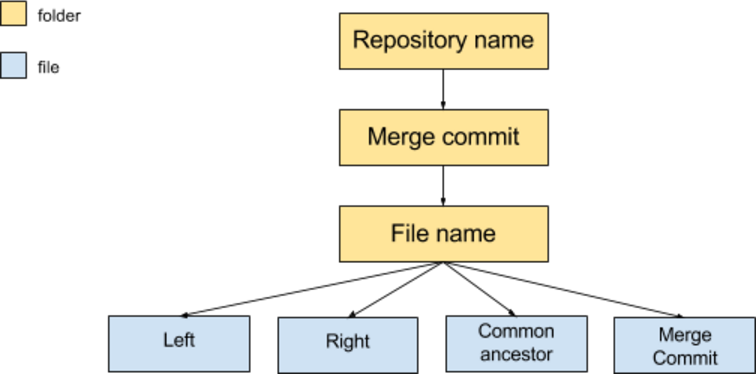
\includegraphics[width=0.45\linewidth, trim=3cm 11cm 3cm 11cm]{figure/conflicts.png}
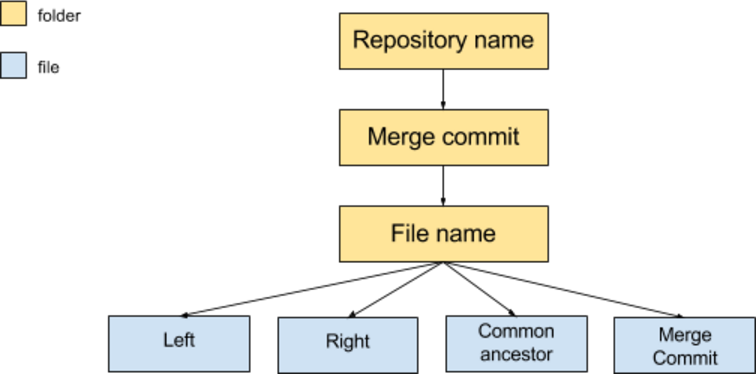
\includegraphics[width=400pt]{figure/conflicts.png}
\caption{Structure of a Conflict File Tree}
\end{figure}

Having all the conflicting file versions in a structured manner made it easier to manually analyze how git conflicts look like in files. Using the command:
\lstset{language=Bash,numbers=left,xleftmargin=2em,frame=single,framexleftmargin=1.5em}
\begin{lstlisting}[frame=single]
git merge-file -p --diff3 <left> <ancestor> <right>
\end{lstlisting}
We got the conflict output from git when merging the specified files \textit{left} and \textit{right}. Looking at the output manually on some of the conflicts, and thereafter looking at the resulting file, we saw that on some cases, they chose the version of the conflict that contained every line of the version that was not chosen plus some additional code. We thought it would be interesting to investigate this further by looking at more examples from the output of Conflicts Analyzer.

\section{Classify Merge Conflicts}
To classify conflicts, we used the tool Conflicts Analyzer developed by Accioly(source). The tool produces a conflict report with information of each conflict of a specified project. We extended the tool to add the additional information Merge commit hash, Parent 1 hash and Parent 2 hash. Due to that the tool uses another merge technique than git, it finds conflicts that was not a conflict in Git. As we are interested in how the developers themselves solves conflicts, we are not interested in such conflicts. Therefore we also modified the tool to only analyze conflicts from merges that also yields a conflict when merged by Git. We did this by reusing our code that re-creates merges (see section Conflict File Tree).

The output in the conflict report contains the the following information:
\begin{itemize}
\item Conflict type
\item Merge Commit hash
\item Parent1 hash
\item Parent2 hash
\item Number of Conflicts
\item Conflict body
\item File path
\end{itemize}

\section{Manual Analysis}
When manually analyzing the output of Conflicts Analyzer we found that it may be possible to find resolution patterns for the Conflict-categories SameSignatureCM and EditSameMC by comparing the two versions with the result. These categories mean that two versions exist for the same method or constructor. For SameSignatureCM, two different versions of the method or constructor was added ie. the method did not exist in the common ancestor. For EditSameMC, the method existed in the common ancestor but was modified in both versions.

26 different examples of conflicts from 9 different projects in the conflict pattern SameSignatureCM were examined. These projects were Atmosphere, Activiti, Blueprints, BroadLeadCommerce, Buildcraft, EventBus, android-async-http, RxJava, Elasticsearch. For each conflict, we looked at the two versions of the method or constructor, and tried to understand why they chose the one they did. What do the versions they chose have in common?

To do this, we proposed some categories which we wanted to check in a quantitative analysis.
\begin{table}
\begin{tabular}{ p{8cm} p{6cm} }
\hline
\multicolumn{1}{c}{\textbf{Category}} & \multicolumn{1}{c}{\textbf{Description}}\\
Recent & The result is equal to the most recent version\\
Superset & The result is a superset of the code in both versions\\
Subset & The result is a subset of the code in both versions\\
Keywords & The result is equal to the version which contains more instances of specific keywords\\
\end{tabular}
\caption{Proposed categories}\label{table:pcategories}
\end{table}
To be able to analyze conflicts parsed by the Conflict Analyzer tool, a script was written in Bash to automatically extract the Java-files that conflicted in the merge, as well as the common ancestor file and the resolution file after the merge was made.

To extract the files, the script first resets the git repository so that HEAD points to the same commit as the latest commit on the remote master branch. The output from Conflicts Analyzer has stripped down the commit hash, hence, the script parses the full commit hash of the parents from the git log. From the git log, the hash of the merge commit is also parsed. Using the git command:
\lstset{language=Bash}
\begin{lstlisting}[frame=single]
git --no-pager log --merges --format=%p <hash> | head -n1
\end{lstlisting}
where \textit{hash} is the merge commit hash. We then parse the two commits and performs the merge using the following sequence of commands:\\
\lstset{language=Bash,numbers=left,xleftmargin=2em,frame=single,framexleftmargin=1.5em}
\begin{lstlisting}[frame=single]
git merge-base <C1> <C2>
\end{lstlisting}
Where \textit{C1} and \textit{C2} refers to the hashes of the parents.  Then, the two parent commits, the merge commit and the common ancestor commit  are checked out respectively and the desired file is copied to a specified output folder. Finally, the script parses the date of the parent commits and prints it to a file in the specified output folder.

Manual analysis of the extracted files were made to see whether the categories described above would emerge repeatedly in many resolutions. A spreadsheet were created and 26 cases were analyzed. The data gathered in the spreadsheet consisted of Project name, Function name, Merge hash, Merge commit message, Parent1 hash, Parent2 hash, Parent1 date, Parent2 date, Conflict pattern, Resolution categories, Comment.

\section{Automatic Tool}
To conduct a large scale analysis we developed a tool that reads the output of ConflictsAnalyzer. The tool then filters out those conflicts we are interested in. Those conflicts are then analyzed and the result is printed in a spreadsheet.

From the qualitative analysis, we saw that sometimes the version that is chosen has more if-statements than the other version. We decided that it would be interesting to see whether choosing such a version reoccurs in many cases. It would also be interesting to see other cases where the version chosen had more of error handling and log printouts. Therefor, we proposed a list of keywords to search for in the versions. The keywords we want to search for are:
\begin{itemize}
\item if
\item log
\item print
\item try
\end{itemize}

\subsection{Input}
We use the data from ConflictsAnalyzer as input for our tool. The tool filters out every conflict that is not of the type SameSignatureCM or EditSameMC. It also removes conflicts in which any version of the function is empty, ie. the function was removed in one version. Conflicts that contain obscure output data from ConflictsAnalyzer, such as if the conflict is not a git conflict, are also skipped.

From the “Conflict body” in the output, the name and signature of the conflicting function is parsed, as well as the parameter types that the function takes. The function body of the two versions in “Conflict body” is also parsed. This information is stored, and using the function name and the parameter types the function takes, the tool is able to parse the resolution function in the merge-commit by checking the commit out and read the specified Java file from “File path”.

This information is then used to find the result from the resolution function in the merge-commit. The different versions of the function are extracted and saved. To filter out the conflicts that arose only due to different spacing or new lines on different places, each line in the extracted functions are trimmed and empty lines are removed. The conflicts, in which the conflicting versions of the function thereafter are equal, are removed.

\subsection{Classifying Conflict-Resolutions}
The left and right version of the function is now compared to the function in the result. First they are checked for equality, ie. is the result equal to the left, right, both or none of the versions.

We are also interested to see if the result is a superset or intersection of the code in the left and right versions. Consider the following example of a superset:

Left version:
\lstset{language=Java,numbers=left,xleftmargin=2em,frame=single,framexleftmargin=1.5em}
\begin{lstlisting}[frame=single]
private int getValue(int index) {
	return (index >= values.size()) ? -1 : values[index];
}
\end{lstlisting}

Right version:
\lstset{language=Java,numbers=left,xleftmargin=2em,frame=single,framexleftmargin=1.5em}
\begin{lstlisting}[frame=single]
private int getValue(int index) {
	return values[index];
}
\end{lstlisting}

The left version contains all code from the right version plus a check for the index size. To detect that this is a superset it is not enough to compare them by line. We solved this by instead considering the set of words in the code. All code in the left and right versions are therefore split into words and added to a hashset. The result code is then also split. The result is a superset if and only if the set of words in the result is equal to the set of all words in the left and right code. To check for intersection, the left and right versions are split into words and put in two separate sets. The result is an intersection if and only if the intersection of the two sets is equal to the set of words in the result.

Then, the tool extracts the commit date of the parents to see if the chosen version was the most recent one. The date of the commits are extracted using the command:
\lstset{language=Bash,numbers=left,xleftmargin=2em,frame=single,framexleftmargin=1.5em}
\begin{lstlisting}[frame=single]
git log -1 <hash> --format=%ci
\end{lstlisting}

Lastly, for each version of the method or constructor, we calculate the number of occurrences of each keyword.




